\section{Álgebra lineal}
\subsection{Notación general}
Se denota un \textbf{vector} $\vec{x}$ como $x \in \mathbb{R}^n$ con $n$ entradas, donde $x_i \in \mathbb{R}$ es la entrada i-ésima. Un vector se puede ver como una matriz de dimensiones $n \times 1$ y se denomina también como vector-columna.
$$\vec{x} = \begin{pmatrix}
x_1 \\ x_2 \\ ... \\ x_n
\end{pmatrix} \in \mathbb{R}^n$$

Se denota una \textbf{matriz} $\vec{A}$ como $A \in \mathbb{R}^{m \times n}$ con n columnas y m filas, donde $A_{i,j} \in \mathbb{R}$ es la entrada en la fila i-ésima y columna j-ésima.
$$\vec{A} = \begin{pmatrix}
A_{1,1} & ... & A_{1,n} \\
... & & ...\\
A_{m,1} & ... & A_{m,n}
\end{pmatrix} \in \mathbb{R}^{m \times n}$$

Una \textbf{matriz de identidad} $\vec{I} \in \mathbb{R}^{n \times n}$ es una matriz cuadrada con 1 en la diagonal principal y 0 en el resto. Para cualquier matriz $\vec{A} \in \mathbb{R}^{n \times n}$, se cumple que $\vec{A} \times \vec{I} = \vec{I} \times \vec{A} = \vec{A}$.
$$\vec{I} = \begin{pmatrix}
1 & 0 & ... & 0 \\
0 & 1 & ... & ... \\
... & ... & 1 & 0 \\
0 & ... & 0 & 1
\end{pmatrix}$$

\subsection{Operaciones de matrices}
\paragraph{Multiplicación vector-vector}
Hay dos tipos de productos vector-vector:
\begin{itemize}
\item \textbf{Producto interno (inner product):}
Dados dos vectores $\vec{x},\vec{y} \in \mathbb{R}^n$ de la misma dimensión, el producto interno es un escalar (un sólo número). Se usa en cálculos que involucran proyecciones, determinación de ortogonalidad, etc. El producto interno puede aplicarse en cualquier dimensión.
$$\vec{x}^T y = \sum^n_{i=1} x_iy_i \in \mathbb{R} $$

\item \textbf{Producto externo (outer product):}
Dados dos vectores, no necesariamente de la misma dimensión, $\vec{x} \in \mathbb{R}^m, \vec{y} \in \mathbb{R}^n$, el producto externo es una matriz de $m \times n$.
$$xy^T = \begin{pmatrix}
x_1 y_1 & ... & x_1 y_n \\
...  & & ... \\
x_m y_1 & ... & x_m y_n
\end{pmatrix} \in \mathbb{R}^{m \times n}$$

El producto externo tiene las siguientes aplicaciones en bioinformática:
\begin{itemize}
\item \textbf{Álgebra lineal}
\begin{itemize}
\item \textbf{Matrices de Covarianza}: Se utiliza en la construcción de matrices de covarianza, que son fundamentales en estadística y análisis de datos.
\item \textbf{Representación de Transformaciones}: Ayuda a representar transformaciones lineales y rotaciones en el espacio.
\end{itemize}
\item \textbf{Análisis de Datos y Machine Learning}
\begin{itemize}
\item \textbf{Modelos de Regresión}: En algunos métodos de regresión, como la regresión de mínimos cuadrados, se utiliza el producto externo para construir matrices de diseño.
\item \textbf{Métodos de Factorización}: Se aplica en técnicas como la factorización de matrices y la descomposición en valores singulares (SVD), que son esenciales en la reducción de dimensionalidad y análisis de componentes principales (PCA).
\end{itemize}
\end{itemize}
\end{itemize}

\paragraph{Multiplicación matriz-vector} Dada una matriz $\vec{A} \in \mathbb{R}^{m \times n}$ y un vector $\vec{x} \in \mathbb{R}^n$, el producto es un vector del tamaño $\mathbb{R}^m$. El proceso consiste en multiplicar cada fila de la matriz $\vec{A}$ por el vector $\vec{x}$ y sumar los resultados.
$$Ax = \begin{pmatrix}
A_{1,1}x_1 + A_{1,2}x_2 + ... + A_{1,n}x_n \\
... \\
A_{m,1}x_1 + A_{m,2}x_2 + ... + A_{m,n}x_n
\end{pmatrix} \in \mathbb{R}^m$$

\begin{figure}[h]
\centering
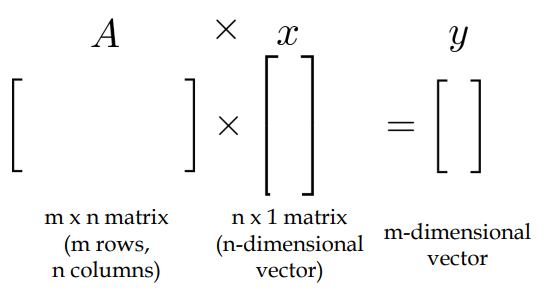
\includegraphics[width = 0.5\textwidth]{figs/matrix-vector-mult.png}
\end{figure}

Entre las aplicaciones de la multiplicación matriz-vector se encuentran:
\begin{itemize}
\item \textbf{Álgebra lineal y matemáticas puras}
\begin{itemize}
\item \textbf{Sistemas de Ecuaciones Lineales}: Resolver sistemas de ecuaciones de la forma $Ax = b$.
\item \textbf{Transformaciones Lineales}: Representar y aplicar transformaciones lineales como rotaciones, escalamientos y reflexiones.
\end{itemize}
\item \textbf{Computación y Algoritmos}
\begin{itemize}
\item \textbf{Algoritmos de Optimización}: Implementar métodos de optimización como gradiente descendente.
\item \textbf{Análisis de Gráficos}: Procesar datos en grafos y redes, como algoritmos de PageRank.
\item \textbf{Compresión de Datos}: Utilizar en algoritmos de compresión de datos y análisis de componentes principales (PCA).
\end{itemize}
\item \textbf{Machine Learning e Inteligencia Artificial}
\begin{itemize}
\item \textbf{Regresión Lineal}: Resolver problemas de regresión lineal para ajustar modelos a datos.
\item \textbf{Redes Neuronales}: Calcular activaciones y actualizar pesos en redes neuronales.
\end{itemize}
\item \textbf{Bioinformática}
\begin{itemize}
\item \textbf{Análisis de Datos Genómicos}: Procesar y analizar grandes volúmenes de datos genómicos y de secuenciación.
\end{itemize}
\end{itemize}

\paragraph{Multiplicación matriz-matriz} Dadas dos matrices $\vec{A} \in \mathbb{R}^{m \times n}$ y $\vec{B} \in \mathbb{R}^{n \times p}$, el producto es una matriz de tamaño $\mathbb{R}^{m \times p}$.
$$\vec{AB} = \begin{pmatrix}
\sum^n_{k=1}A_{1,k}B_{k,1} & ... & \sum^n_{k=1}A_{1,k}B_{k,p} \\
... & ... & ...\\
\sum^n_{k=1}A_{m,1}B_{k,1} & ... & \sum^n_{k=1}A_{m,k}B_{k,p}
\end{pmatrix} \in \mathbb{R}^{m \times p}$$

\begin{figure}[h]
\centering
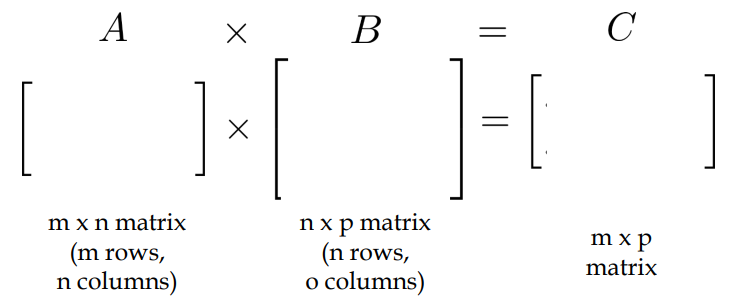
\includegraphics[width = 0.7\textwidth]{figs/matrix-matrix-mult.png}
\end{figure}

\subsection{Propiedades de la multiplicación de matrices}
\paragraph{No conmutatividad:} En general, la multiplicación de matrices no es conmutativa, es decir, $\vec{A} \times \vec{B} \neq \vec{B} \times \vec{A}$. Por ejemplo:
$$\begin{bmatrix}
1 & 1 \\ 0 & 0
\end{bmatrix} \times \begin{bmatrix}
0 & 0 \\ 2 & 0
\end{bmatrix} = \begin{bmatrix}
2 & 0 \\ 0 & 0
\end{bmatrix} $$

$$\begin{bmatrix}
0 & 0 \\ 2 & 0
\end{bmatrix} \times \begin{bmatrix}
1 & 1 \\ 0 & 0
\end{bmatrix} = \begin{bmatrix}
0 & 0 \\ 2 & 2
\end{bmatrix} $$

En el caso de multiplicar una matriz con una matriz de identidad, sí es conmutativa.

\paragraph{Matriz inversa} Si $\vec{A}$ es una matriz cuadrada $m \times m$, y tiene inversa, entonces
$$AA^{-1} = A^{-1}A = I$$

\paragraph{Transposición de matriz} Dada una matriz $A \in \mathbb{R}^{m \times n}$, su transpuesta $A^T$: es una matriz $n \times m$ donde $\forall i, j, \quad (A^T)_{ij} = A_{ji}$. Por ejemplo:
\begin{table}[h]
\centering
$A = \begin{bmatrix}
1 & 2 & 0 \\ 3 & 5 & 9
\end{bmatrix}$
\qquad \qquad \qquad
$A^T = \begin{bmatrix}
1 & 3 \\ 2 & 5 \\ 0 & 9
\end{bmatrix} $
\end{table}
% Luis -> meter el resto de operaciones y propiedades de https://stanford.edu/~shervine/teaching/cs-229/refresher-algebra-calculus (el finde quizá?).